%==========================================================================
%  TRES0312 Fysikk — Foiler-mal
%
%  MØrk/lys modus: kommenter ut én av de to linjene nedenfor.
%==========================================================================
\newif\ifdarkmode
\darkmodetrue      % ← mørk modus
%\darkmodefalse   % ← lys modus  (fjern % foran og legg % foran linjen over)

\documentclass[aspectratio=169, 12pt]{beamer}

\usepackage{amd-beamer}

%--------------------------------------------------------------------------
%  DOKUMENTINFO
%--------------------------------------------------------------------------
\title{Tall i fysikk!}
\subtitle{TRES0312 --- Signifikante siffer og standardform}
\author{Ben David Normann}
\date{\today}

%--------------------------------------------------------------------------
%  SEKSJONSKONTEKST
%  \setcounter{section}{N} setter gjeldende seksjonsnummer til N, slik at
%  \defn, \exm og \oppgave får samme nummerering som i kompendiet.
%  Tellerne nullstilles automatisk ved hvert \setcounter{section}{...}.
%  Bruk gjerne \setcounter{section}{N} rett før en frame der du bytter
%  seksjon, i stedet for én gang globalt.
%--------------------------------------------------------------------------
\setcounter{section}{3}   % Seksjon 3: "Signifikante siffer"

\begin{document}

%--------------------------------------------------------------------------
%  SLIDE 1 — TITTELSIDE
%--------------------------------------------------------------------------
\begin{frame}[plain]
  \titlepage
\end{frame}


%--------------------------------------------------------------------------
%  SLIDE 2 — Tre kjappe fra forrige gang
%--------------------------------------------------------------------------

\begin{frame}{}

  \repetisjon{Tre kjappe fra forrige gang}{%
    \begin{enumerate}[1.,itemsep=10pt]
      \item Hva er en fysisk størrelse?
      \item Hva er de 7 SI-enhetene?
      \item Gjør om $250\,\mathrm{cm}$ til meter.
    \end{enumerate}
  }

\end{frame}

%--------------------------------------------------------------------------
%  SLIDE 3 — Sau og sort hull
%--------------------------------------------------------------------------

\begin{frame}{Målenøyaktighet}

  \begin{columns}[t]
    \begin{column}{0.48\textwidth}
      \begin{center}
        \ifdarkmode
          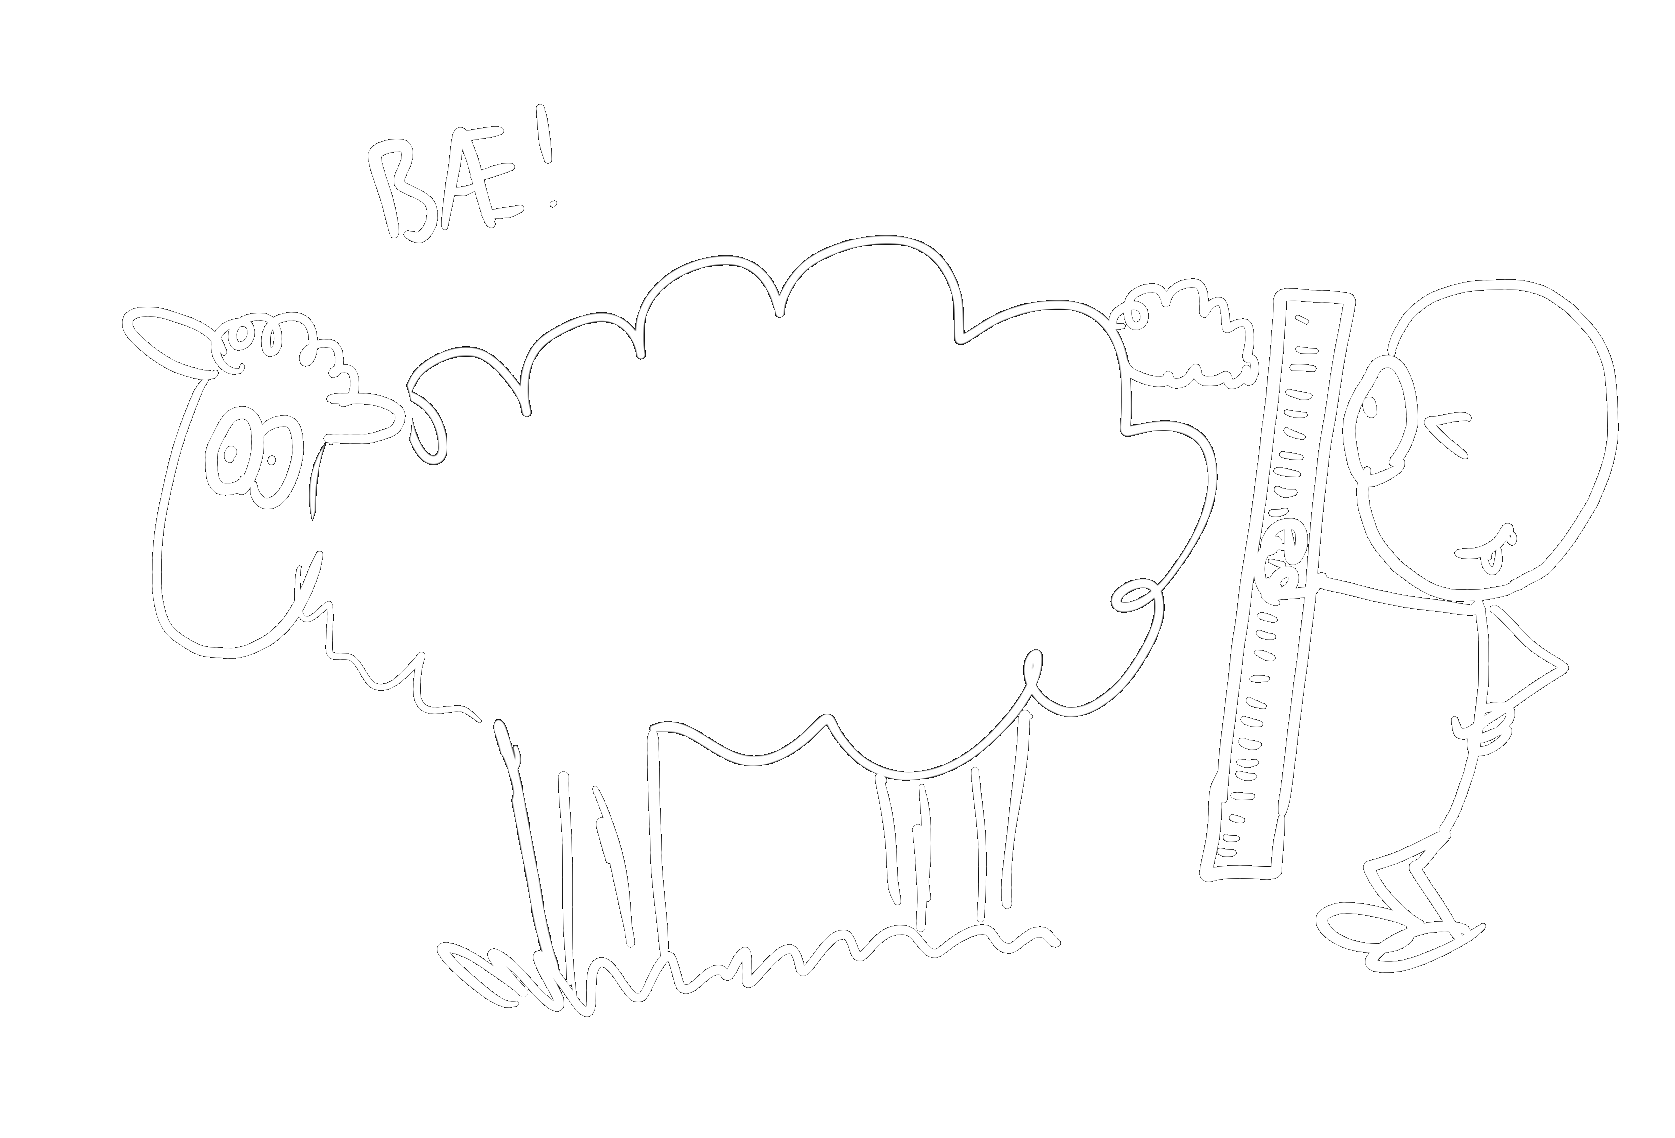
\includegraphics[width=\textwidth]{Images/sau_maling_mork.png}
        \else
          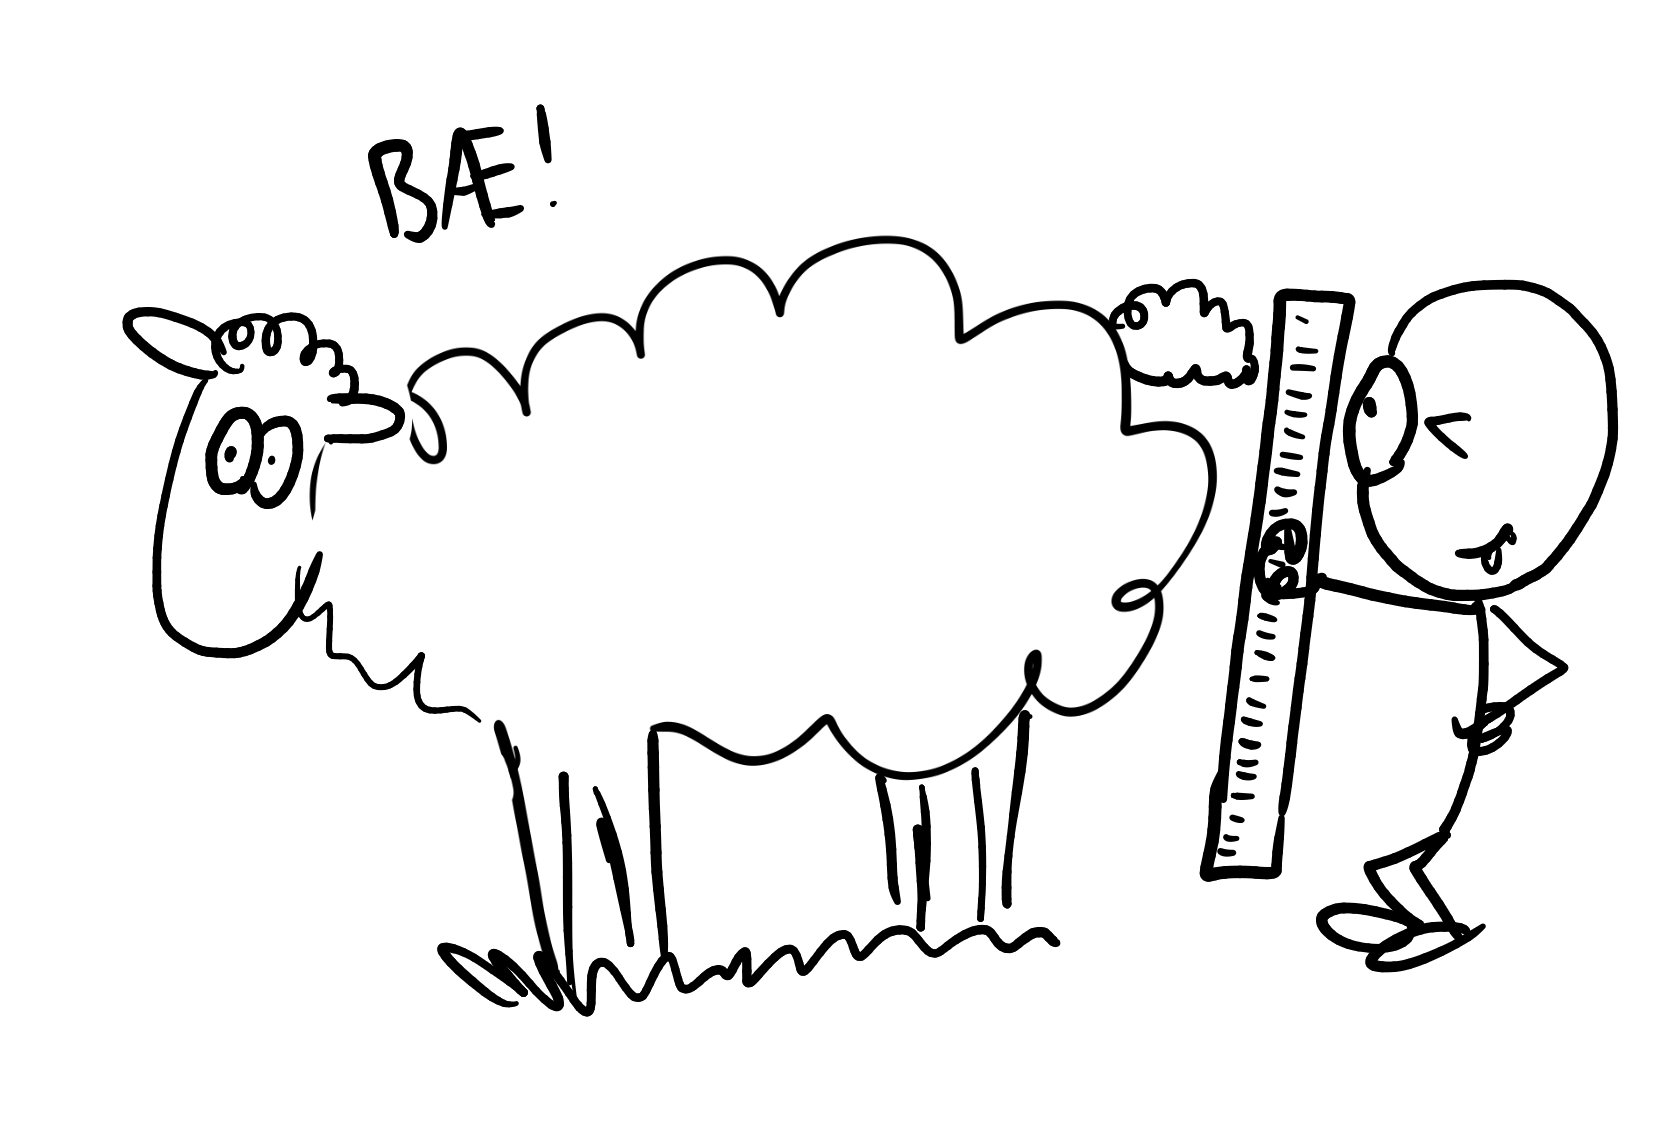
\includegraphics[width=\textwidth]{Images/sau_maling_lys.png}
        \fi
      \end{center}
    \end{column}
    \pause
    \begin{column}{0.48\textwidth}
      \begin{center}
        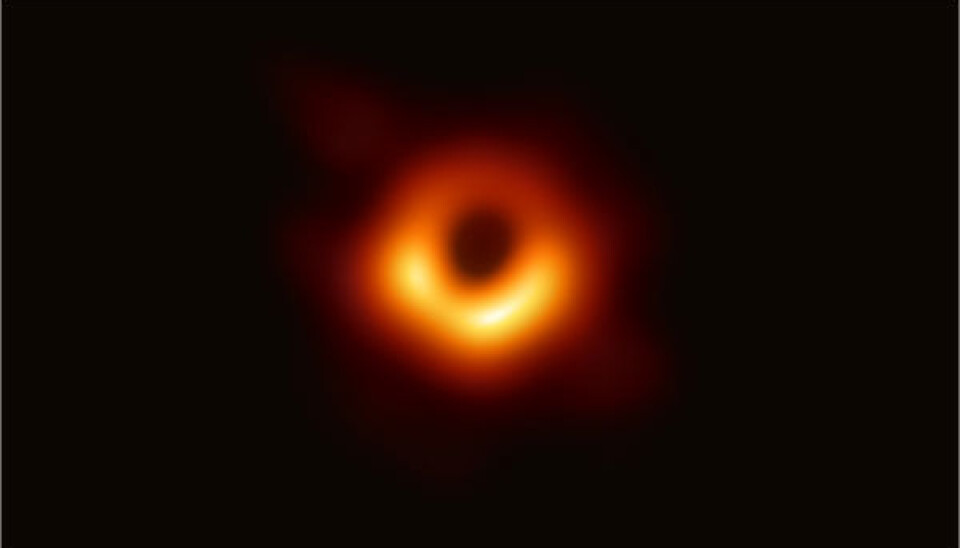
\includegraphics[width=\textwidth]{Images/sort_hull_ekte.png}
      \end{center}
    \end{column}
  \end{columns}

\end{frame}

%--------------------------------------------------------------------------
%  SLIDE 4 — Avrunding
%--------------------------------------------------------------------------

\begin{frame}{Målenøyaktighet (signifikans) og avrunding}
\oppsum{Signifikante siffer}{%
    \begin{itemize}
        \item Antall signifikante siffer regnes fra første tall forskjellig fra null.
        \item I en utregning skal svaret angis med samme nøyaktighet (antall siffer) som den \textit{minst nøyaktige} størrelsen som inngikk i beregningen.
    \end{itemize}
}
\oppsum{Avrunding}{%
Vi minner om følgende regler for avrunding:
\begin{itemize}
    \item Tall fra 0-4 rundes ned. Tall fra og med 5 til 9 rundes opp.
    \item Avrunding til riktig antall signifikante siffer må skje helt tilslutt i en beregning!
\end{itemize}
}
\end{frame}

%--------------------------------------------------------------------------
%  SLIDE 5 — Signifikante siffer
%--------------------------------------------------------------------------
\begin{frame}{}
  \aktivitet{Beregning av areal}{%
En rektangulær hage har lengde $L = 12.3\,\mathrm{m}$ og bredde $B = 4.56\,\mathrm{m}$. Hva er arealet av hagen? Oppgi svaret med riktig antall signifikante siffer.
}
\end{frame}

%--------------------------------------------------------------------------
%  SLIDE 6 — Eksempel: Signifikante siffer
%--------------------------------------------------------------------------
\begin{frame}{Aktivitet}
  \aktivitet{Eksempel 1.6: Signifikante siffer}{%
    Hvor mange signifikante siffer har tallene
    \begin{enumerate}[a)]
      \item $165.00$
      \item $0.791400$
      \item $14$
    \end{enumerate}
  }
  \aktivitet{Eksempel 1.7: Signifikante siffer i utregning}{%
    Eline kjører $5.00\,\mathrm{km}$ på $6.0$ minutter. Hvor fort kjører hun i gjennomsnitt?
  }
\end{frame}

\begin{frame}{Tall på standardform}
Standardform er en måte å skrive tall på som tydeliggjør både antall siffer og størrelsesorden.
\[
\textrm{T}=t \cdot 10^n,
\]
\aktivitet{Standardform}{%
\begin{enumerate}[a)]
    \item Skriv $0.000000000000000000000000001$ på standardform.
    \item Skriv $123\,000\,000\,000$ på standardform.
    \item Regn ut $1.23 \times 10^8 \div 4.56 \times 10^3$ og oppgi svaret med riktig antall signifikante siffer.
    \item Regn ut $7.89 \times 10^{-5} \cdot 1.23 \times 10^4$ og oppgi svaret med riktig antall signifikante siffer.
\end{enumerate}
}

\end{frame}

%--------------------------------------------------------------------------
%  SLIDE 7 — Eksempel: Standardform
%--------------------------------------------------------------------------
\begin{frame}{Aktivitet}
  \aktivitet{Eksempel 1.8: Standardform}{%
    Skriv følgende tall på standardform:
    \begin{enumerate}[a)]
      \item $0.07$
      \item $112$
      \item $56\,700\,000$
    \end{enumerate}
  }
\end{frame}

\begin{frame}{Dekadiske prefikser}
  \begin{center}
  \scriptsize
  \renewcommand{\arraystretch}{1.0}
  \begin{tabular}{|c|l|c|l|}
  \hline
  \rowcolor{blue!10!black!80}
  $10^n$ & Prefiks & Symbol & Navn \\
  \hline
  $10^{24}$ & yotta & Y & kvadrilion \\
  $10^{21}$ & zetta & Z & trilliard \\
  $10^{18}$ & exa   & E & trillion \\
  $10^{15}$ & peta  & P & billiard \\
  $10^{12}$ & tera  & T & billion \\
  $10^{9}$  & giga  & G & milliard \\
  $10^{6}$  & mega  & M & million \\
  $10^{3}$  & kilo  & k & tusen \\
  $10^{2}$  & hekto & h & hundre \\
  $10^{1}$  & deka  & da & ti \\
  $10^{-1}$ & desi  & d & tidel \\
  $10^{-2}$ & centi & c & hundredel \\
  $10^{-3}$ & milli & m & tusendel \\
  $10^{-6}$ & mikro & $\mu$ & milliondel \\
  $10^{-9}$ & nano  & n & milliarddel \\
  $10^{-12}$& piko  & p & billiondel \\
  $10^{-15}$& femto & f & billiarddel \\
  $10^{-18}$& atto  & a & trilliondel \\
  $10^{-21}$& zepto & z & trilliarddel \\
  $10^{-24}$& yocto & y & kvadrilliondel \\
  \hline
  \end{tabular}
  \end{center}
\end{frame}

%--------------------------------------------------------------------------
%  SLIDE 8 — Eksempel: Dekadiske prefikser
%--------------------------------------------------------------------------
\begin{frame}{Aktivitet}
  \aktivitet{Eksempel 1.9: Dekadiske prefikser}{%
    En viruspartikkel har diameter $d = 90\,\mathrm{nm}$.
    \begin{enumerate}[a)]
      \item Skriv diameteren i mikrometer ($\mu\mathrm{m}$).
      \item Skriv diameteren på standardform i meter.
    \end{enumerate}
  }
\end{frame}

%--------------------------------------------------------------------------
%  SLIDE 9 — Pause
%--------------------------------------------------------------------------

\begin{frame}{}
\begin{center}
\Huge{Pause!}
\end{center}
\end{frame}

%--------------------------------------------------------------------------
%  SLIDE 10 — Fart
%--------------------------------------------------------------------------

\begin{frame}{Fart}
  \vspace{-3mm}
  \spq{Hva er fart? Hvordan måles det?}
  \vspace{-3mm}
  \pause
  \svar{
  Fart forteller oss hvor raskt noe beveger seg. Gjennomsnittsfarten til en gjenstand over et tidsrom er den tilbakelagte strekningen delt på tiden det tok:
  \vspace{-2mm}
  \graabox{$\displaystyle \bar{v} = \frac{\Delta s}{\Delta t} = \frac{s_2 - s_1}{t_2 - t_1}$}
  \vspace{-2mm}
  Fart måles for eksempel i meter per sekund (m/s) eller kilometer per time (km/t).
  }
\end{frame}

%--------------------------------------------------------------------------
%  SLIDE 11 — Aktivitet: gjennomsnittlig fart fra posisjonsgraf
%--------------------------------------------------------------------------

\begin{frame}{Aktivitet}
  \vspace{-3mm}
  \aktivitet{Gjennomsnittlig fart fra en posisjonsgraf}{%
  Grafen under viser posisjonen $s$ til en syklist som funksjon av tiden $t$, gitt ved $s(t) = 0.5t^2 + 2t$ (med $s$ i meter og $t$ i sekunder).
  \vspace{-2mm}

  \begin{center}
  \begin{tikzpicture}
  \begin{axis}[
    kinemplot, height=3.3cm, width=0.68\textwidth,
    xlabel={Tid $t$ [s]},
    ylabel={Posisjon $s$ [m]},
    xmax=6, ymin=0, ymax=32,
    xtick={0,1,2,3,4,5,6}, ytick={0,10,20,30},
  ]
    \addplot[thick, posGraphColor, domain=0:6, samples=60] {0.5*x^2 + 2*x};
    \addplot[only marks, mark=*, mark size=1.6pt, posGraphColor] coordinates {(1,2.5) (5,22.5)};
    \draw[dashed, textcolor!45] (axis cs:1,0) -- (axis cs:1,2.5) -- (axis cs:0,2.5);
    \draw[dashed, textcolor!45] (axis cs:5,0) -- (axis cs:5,22.5) -- (axis cs:0,22.5);
  \end{axis}
  \end{tikzpicture}
  \end{center}
  \vspace{-2.5mm}

  {\small Ved $t_1{=}1\,$s er $s_1{=}2.5\,$m, og ved $t_2{=}5\,$s er $s_2{=}22.5\,$m. Finn gjennomsnittsfarten mellom $t_1$ og $t_2$ (og evt. momentanfarten ved $t{=}3\,$s, om du kan derivere).}
  }
\end{frame}

%--------------------------------------------------------------------------
%  SLIDE 12 — Akselerasjon
%--------------------------------------------------------------------------

\begin{frame}{Akselerasjon}
  \spq{Hva er akselerasjon? Hvordan måles det?}
  \pause
  \svar{
  Akselerasjon er endringen av farten over tid. Gjennomsnittsakselerasjonen til en gjenstand over et tidsrom er da:
  \graabox{$\displaystyle \bar{a} = \frac{\Delta v}{\Delta t} = \frac{v_2 - v_1}{t_2 - t_1}$}
  Akselerasjon måles for eksempel i meter per sekund i annen (m/s\textsuperscript{2}).
  }
\end{frame}

%--------------------------------------------------------------------------
%  SLIDE 13 — Aktivitet: gjennomsnittlig akselerasjon fra måledata
%--------------------------------------------------------------------------

\begin{frame}{Aktivitet}
  \aktivitet{Gjennomsnittlig akselerasjon fra målte farter}{%
  Tabellen under viser farten til en bil, målt ved noen ulike tidspunkt.
  \begin{center}
  \renewcommand{\arraystretch}{1.3}
  \begin{tabular}{|c|c|c|c|c|c|}
  \hline
  \rowcolor{blue!10!black!80}
  Tid $t$ [s] & 0 & 1 & 2 & 3 & 4 \\
  \hline
  Fart $v$ [m/s] & 2 & 5 & 8 & 11 & 14 \\
  \hline
  \end{tabular}
  \end{center}
  \vspace{1mm}
  Bruk tabellen til å finne bilens gjennomsnittsakselerasjon mellom $t=1\,$s og $t=4\,$s.
  }
\end{frame}

%--------------------------------------------------------------------------
%  SLIDE 14 — Aktivitet: Fart og akselerasjon fra måledata
%--------------------------------------------------------------------------
\begin{frame}{Aktivitet}
  \aktivitet{Fart og akselerasjon fra målte posisjoner}{%
  Tabellen under viser posisjonen til en gjenstand, målt med jevne mellomrom (hvert sekund).
  \begin{center}
  \renewcommand{\arraystretch}{1.3}
  \begin{tabular}{|c|c|c|c|c|c|c|}
  \hline
  \rowcolor{blue!10!black!80}
  Tid $t$ [s] & 0 & 1 & 2 & 3 & 4 & 5 \\
  \hline
  Posisjon $s$ [m] & 0 & 2 & 5 & 9 & 14 & 20 \\
  \hline
  \end{tabular}
  \end{center}
  \vspace{1mm}
  Bruk Python til å regne ut og plotte gjennomsnittsfarten og gjennomsnittsakselerasjonen til gjenstanden, mellom hvert måletidspunkt.
  }
\end{frame}

\begin{frame}
\begin{center}
  \Huge{Neste gang: Kapittel 2 — Matematikk vi trenger!}
  \begin{itemize}
    \item Grunnleggende algebra
    \item Trigonometri
    \item Vektorer
  \end{itemize}
\end{center}
\end{frame}


\end{document}
